\emph{A previous version of this chapter was published in
\citet{CharltonLeichKaddoura2021avoev}.}

Augmenting or even replacing fixed-route transit lines with automated, connected, shared taxi fleets may be a desirable alternative in less-densely developed areas. The MATSim agent-based transport microsimulation model is used to study scenarios including the status quo, dynamically-dispatched fleets with drivers, and fully autonomous fleets.

This chapter describes a unique, web-based data visualization portal for investigating aspects of shared-taxi fleet scenarios, developed for use by researchers and public transit agencies. The data visualization portal includes many interactive views such as agent (taxi) movements color-coded by number of passengers and trip request origins and destinations, changes in roadway and passenger volumes compared to a base case, and more. The agent-based simulation covers a 24 hour simulation period; analysts can hone in on specific times of day to examine, e.g. school pickup/drop-offs or commute trips connecting to rail stations.

The tool is in operation for several small cities and rural regions in Germany and was successfully used as an outreach tool in public meetings. In addition, developers of the MATSim DRT extension found the visualizations particularly useful for debugging both the algorithms and the scenario definitions. The code is entirely open source and, while this specific study has a rather esoteric use case, the visualization platform has an extensible design that can be modified for other purposes.

%% ----- INTRODUCTION -----
\section{Introduction}
\label{avov-introduction}

Augmenting or replacing fixed-route transit lines with automated, connected, shared taxi fleets may be a desirable alternative for transit agencies in less-densely developed areas. The economics of fixed-route transit are difficult to square with sparse development patterns, especially with the advent of private ride-hailing services which add the "shared taxi" concept to people's travel options \cite{Hough2018}. The same technologies used by private ride-hailing, however, can also be modified and applied to future transit services.

In this study, known in German as AVÖV\footnote{Automasierter vernetzter öffentlicher Verkehr: Automated, networked public transit}, a new \gls{DRT} shared taxi service is examined as an alternative approach to serving the population of rural areas and less-dense portions of urban regions. Dynamic-response transit is analyzed using the \gls{MATSim} agent-based transport microsimulation model. MATSim is an extensible, activity- and multi-agent based transport simulation, which enables the simulation of large scale scenarios. \cite{MATSimBook}. Crucially, MATSim simulates passenger transport in both private and public modes \cite{ZiemkeEtAl2019OpenBerlinScenario}.

The existing methodology behind using MATSim to simulate DRT is well-described by Bischoff et al \cite{BischoffMaciejewskiNagel2017SharedTaxiIITSC} and is not the focus of this chapter. Rather, in the course of the effort to develop, analyze and compare various DRT scenarios, a need arose to create some truly unique data visualizations that could assist in improving and displaying the DRT scenarios themselves. A web-based portal is the result of this research. The portal is based on the findings of Chapter \ref{ch:mathub} and more directly Chapter \ref{ch:covid-sim}, where a web portal for comparing scenarios was developed for the EpiSim model (described in \cite{MuellerEtAl2021episim}). The scenario comparison portal includes many interactive views, such as taxi movements color-coded by number of passengers and trip request origins and destinations, changes in roadway and passenger volumes compared to a base case, and more. The agent-based simulation covers a 24 hour simulation period; analysts can hone in on specific times of day to examine, e.g. school pickup/drop-offs or commute trips connecting to rail stations.

The tool is in operation for several small cities and rural regions in Germany, and was successfully used as an outreach tool in public meetings online. Project partners at transit agencies are interested in understanding the implications of the DRT simulations, and without a visual component, that would be extremely difficult to provide.

Furthermore, developers of the MATSim DRT extension found the visualizations particularly useful for debugging both the algorithms and the scenario definitions. The latest implementions of MATSim include extensive DRT capabilities whose methods are continually being optimized and improved.

All code for MATSim and the visualization portal is open source and, while this specific study has a quite esoteric use case, the portal has an extensible design that could be modified for other purposes.

%% ----- EXISTING TOOLS AND RESEARCH -----
\section{Motivation: Existing Tools and Research}
\label{avov-motivation}

Agent-based microsimulation is quite complex, producing reams of data and overwhelming details that are not appropriate for stakeholder meetings. PDF reports and PowerPoint slides are the norm in these situations, but building something truly interactive instead could be much more engaging and useful for decision-making.

Many existing tools can analyze agent-based transport simulation outputs. \textbf{OTFVis} \cite{Srippgen2015OTFVisInBook} is a venerable open-source tool designed to integrate tightly with MATSim, however it is not under active development and has neither online features nor DRT-specific capabilities.

The commercial product \textbf{Senozon Via} \cite{Rieser2015SenozonViaInBook} is very feature rich, actively maintained, and is currently used by our research team for myriad internal analysis tasks. It has no online web-based component, although it is very easy to create high-quality screen recordings of simulation results. The lack of interactive options for outreach meetings, as well as Via's focus on advanced analyst tasks, make it a poor fit for outreach despite its many other advantages.

General geographic information system tools, such as \textbf{ArcGis} and its open source corollary \textbf{QGis}, are again very analyst-focused. Unlike QGis, ArcGis can create high quality online dashboards and interactive maps, and the study team has used them in other settings. ArcGis does not have any MATSim-specific capabilities; the rich agent-based details would be entirely lost in the aggregations required to get DRT outputs onto an ArcGis map. ArcGis is also commercial software and was not considered due to the required financial outlay.

Research by \citet{CharltonLaudan2020WebBasedVisualization} described in Chapter \ref{ch:mathub} shows that a web-based tool specific to MATSim is now possible, given the latest advances in graphic technology embedded in modern web browsers. That tool includes a "front-end" website which runs in the user's browser. Through this site the user organizes model outputs, and defines aggregate visualizations for a few typical use cases. The tool also requires a large, complex "back-end" server component which handles file storage, user authentication, output post-processing, and realtime visualization support. That work is an obvious starting point for this research, but for reasons that will be described below, much of it was ultimately discarded.

In summary, the existing tools are all either incapable of visualizing the disaggregate outputs of the DRT module of MATSim in an efficient manner, have no web-based online component, or are inappropriate for anyone except highly trained analysts. Thus the new platform described below is seen as a viable solution.

%% ----- THE PLATFORM -----
\section{The Visualization Platform}
\label{avov-platform}

Despite two years of development of the above-mentioned client/server solution for other studies, problems in the old system were persistent. The two largest: (1) The massive size of MATSim outputs always preclude loading them into a user's web browser; a single DRT run can be 800Mb or more. This forces post-processing and/or aggregation to happen, which can eliminate many of the benefits of a fully disaggregate analysis. (2) The back-end server design requires extensive effort whenever new visualization capabilities are desired. A strict database design and overwrought user/group management capabilities result in a rock-solid system that is unfortunately onerous to modify.

It turns out that complex file and user management is unnecessary.\footnote{This invokes the programming mantra "YAGNI" -- You Aren't Gonna Need It: build the simplest possible solution that works, instead of over-engineering things.} From trial and error and ample iteration emerges a simplified system that eliminates all of the back-end server complexity by eliminating all of the back-end servers:

\begin{itemize}
  \item File storage is delegated to existing servers, instead of creating a special visualization file server. On site, we have an existing "Subversion" server \cite{Collins-SussmanEtc2008SubversionBook} which is adept at large-file storage and version history. All access to the server is via a simple unified interface that can be easily extended to cloud storage, including large offerings such as Amazon S3 or Microsoft Azure
  \item As the site is intended to be publicly accessible, we discard all user authentication capabilities. If you have a web browser, you can view the results of any runs which are stored \emph{in the public area} of the Subversion server. Naturally some parts of file storage remain off-limits to the greater Internet
  \item Analysts define visualizations by creating small configuration text files in the same folder as model outputs. These files include all of the details of a visualization --- usually just a few lines --- pointing to the input files and configuration settings. This eliminates all the hassle of writing code for user interface input dialog boxes.
  \item Post-processing of outputs must be performed by the analyst as part of their modeling workflow, before uploading to Subversion, since browsers cannot ingest MATSim outputs in their entirety. This tool is not an "end-to-end" GUI which lets analysts define, run, and view outputs of their simulations: it is an output viewer.
\end{itemize}

The code is designed as a \gls{SPA} or "single page application" which is a modern way of building Javascript-based websites that behave similarly to desktop applications. Most large consumer-facing websites such as Twitter and Facebook behave in a similar manner, thus this paradigm is easy for end users to understand.

After much trial and error, the platform coalesced around a combination of many different advanced web technologies:

\begin{itemize}
  \item The overall application framework is based on \textbf{VueJS}, a popular Javascript toolkit for building interactive websites. VueJS is the glue between user interface clicks and the application code that runs underneath.
  \item The agent-based visualizations use custom code ("shaders") written using the \textbf{Deck.gl} visualization library
  \item Older visualizations borrowed from Charlton et al's previous research use the \textbf{Mapbox GL} mapping library
  \item Extensive optimization of memory usage for handling these large datasets with the brilliant \textbf{crossfilter} Javascript library\footnote{Crossfilter is available at \href{https://crossfilter.github.io/crossfilter/}{crossfilter.github.io/crossfilter}}, which manages lightning-fast filtering of millions-of-rows datasets in multiple dimensions
\end{itemize}

The entire codebase is open source and is designed with a "plug-in" architecture so that new visualizations can be developed quickly while relying on common infrastructure for common needs such as file access. To create a new visualization, the developer copies an existing template, modifies the Javascript code to take advantage of the Deck.gl or MapBox libraries as needed, and registers it with the main application. End users can then create visualizations by adding corresponding configuration files to a scenario's file server folder.

%% ----- DRT VISUALIZATIONS -----
\section{Dynamic-Response Taxi Visualizations}
\label{avov-drtviz}

Several unique visualizations depict details specific to the dynamic-response transit scenarios in this study. Standard MATSim outputs such as mode shares by time of day, simulation statistics, trip length summaries, and so on are also available in each scenario subfolder.

For best understanding of an interactive website, it is better to view the site in situ than to read the description below. The project site remains online and is better demonstrated than described.\footnote{Site is viewable at \href{https://vsp.berlin/avoev/}{vsp.berlin/avoev}}

\subsection{DRT Animation}

A 24-hour agent-based interactive animation of DRT vehicles traversing the roadway network includes the following features: (1) DRT vehicles traversing the roadway links in real-time, sped up, or in reverse time, for analysis; (2) Vehicles color-coded by occupancy, so users can see the relative amount of ride-sharing occurring at different times of day; (3) Passenger origin/destinations depicted as "flyovers" instead of on the street network, so actual supply and demand can be viewed separately from the roads on which that demand occurs;

Each of these components can be turned on or off to assist in reducing clutter in the animation. The 3D map can be zoomed or panned and its pitch angle adjusted to assist in viewing. Figures \ref{fig:avov-drt-vehicles-routes} and \ref{fig:avov-drt-od} depict snapshots of the DRT animations.

\begin{figure}[ht]
\centering
\begin{minipage}[c]{0.45\textwidth}
   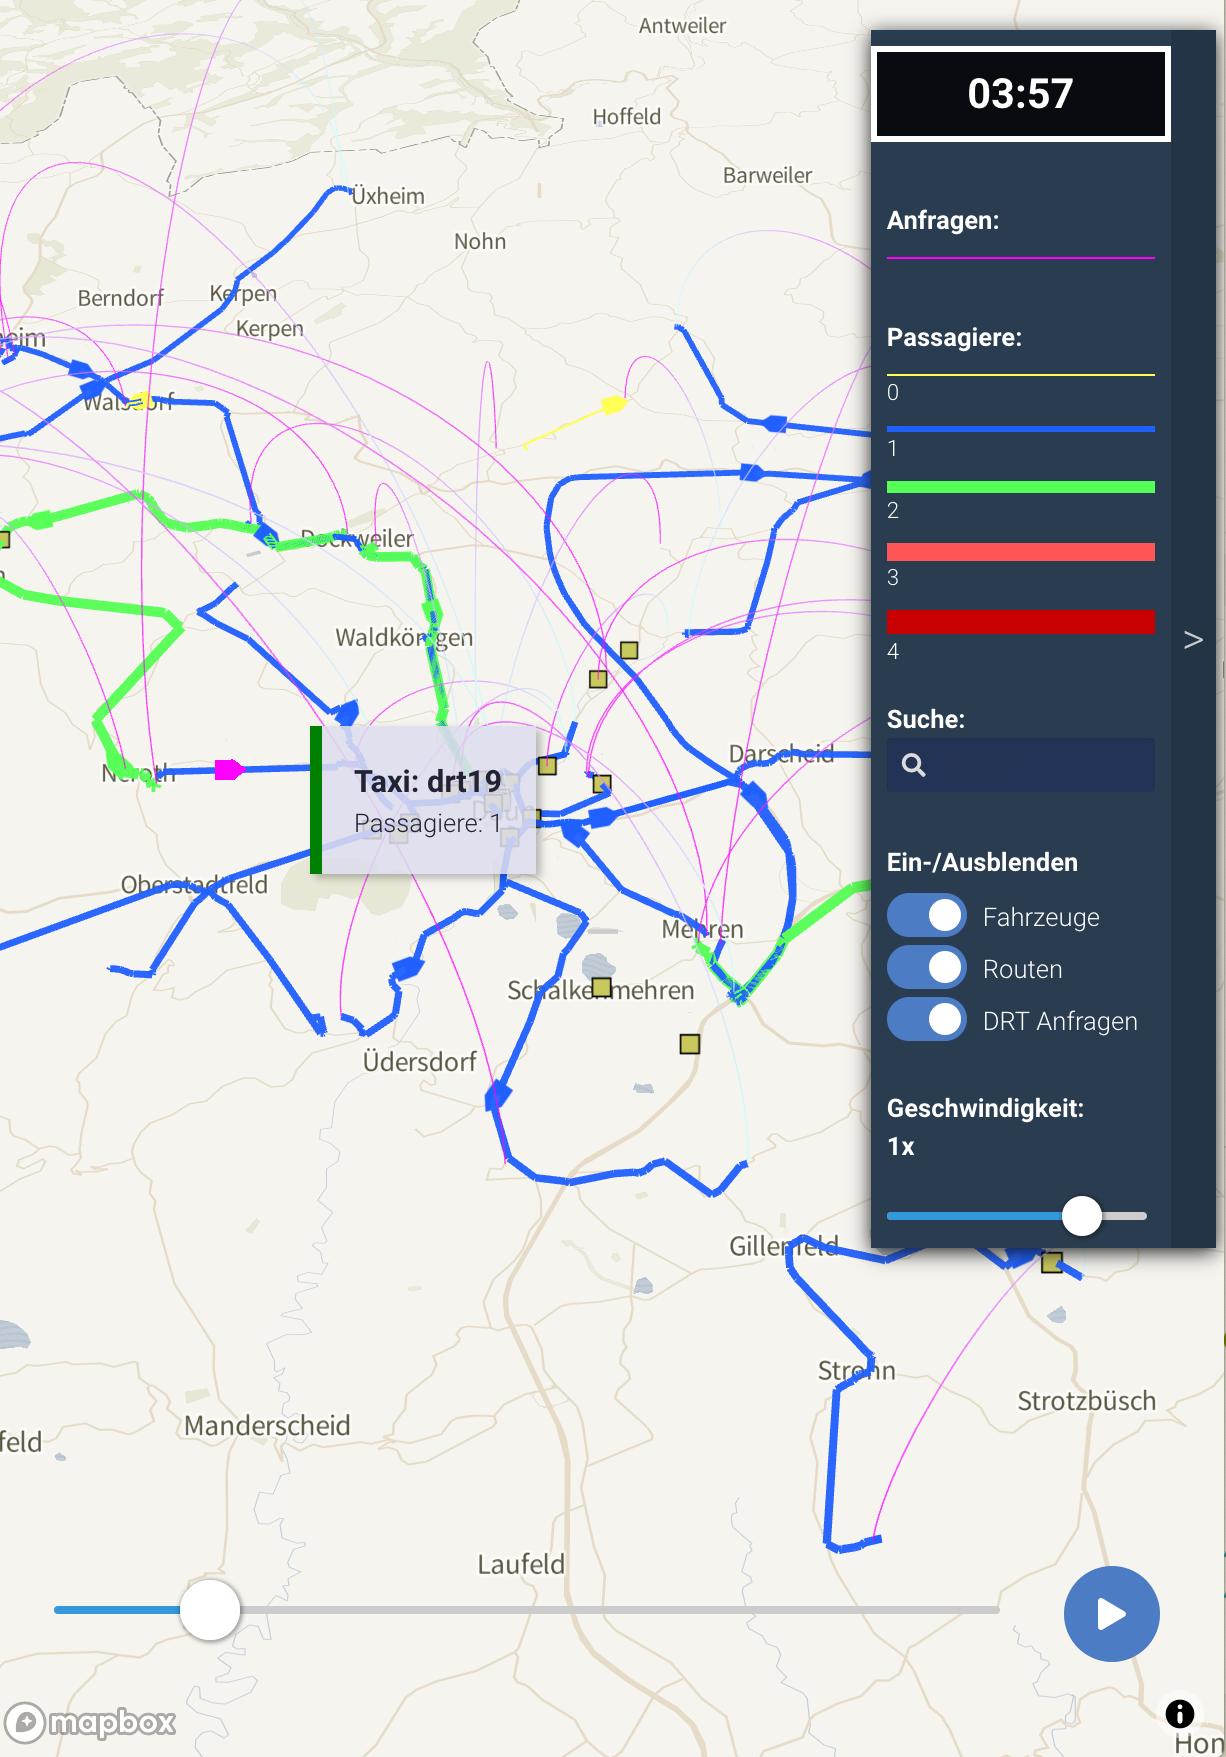
\includegraphics[width=\linewidth]{chapters/22-avov/images/fig-drt-vehicles.png}
   \caption{DRT vehicles and routes}
   \label{fig:avov-drt-vehicles-routes}
\end{minipage}
\begin{minipage}[c]{0.45\textwidth}
   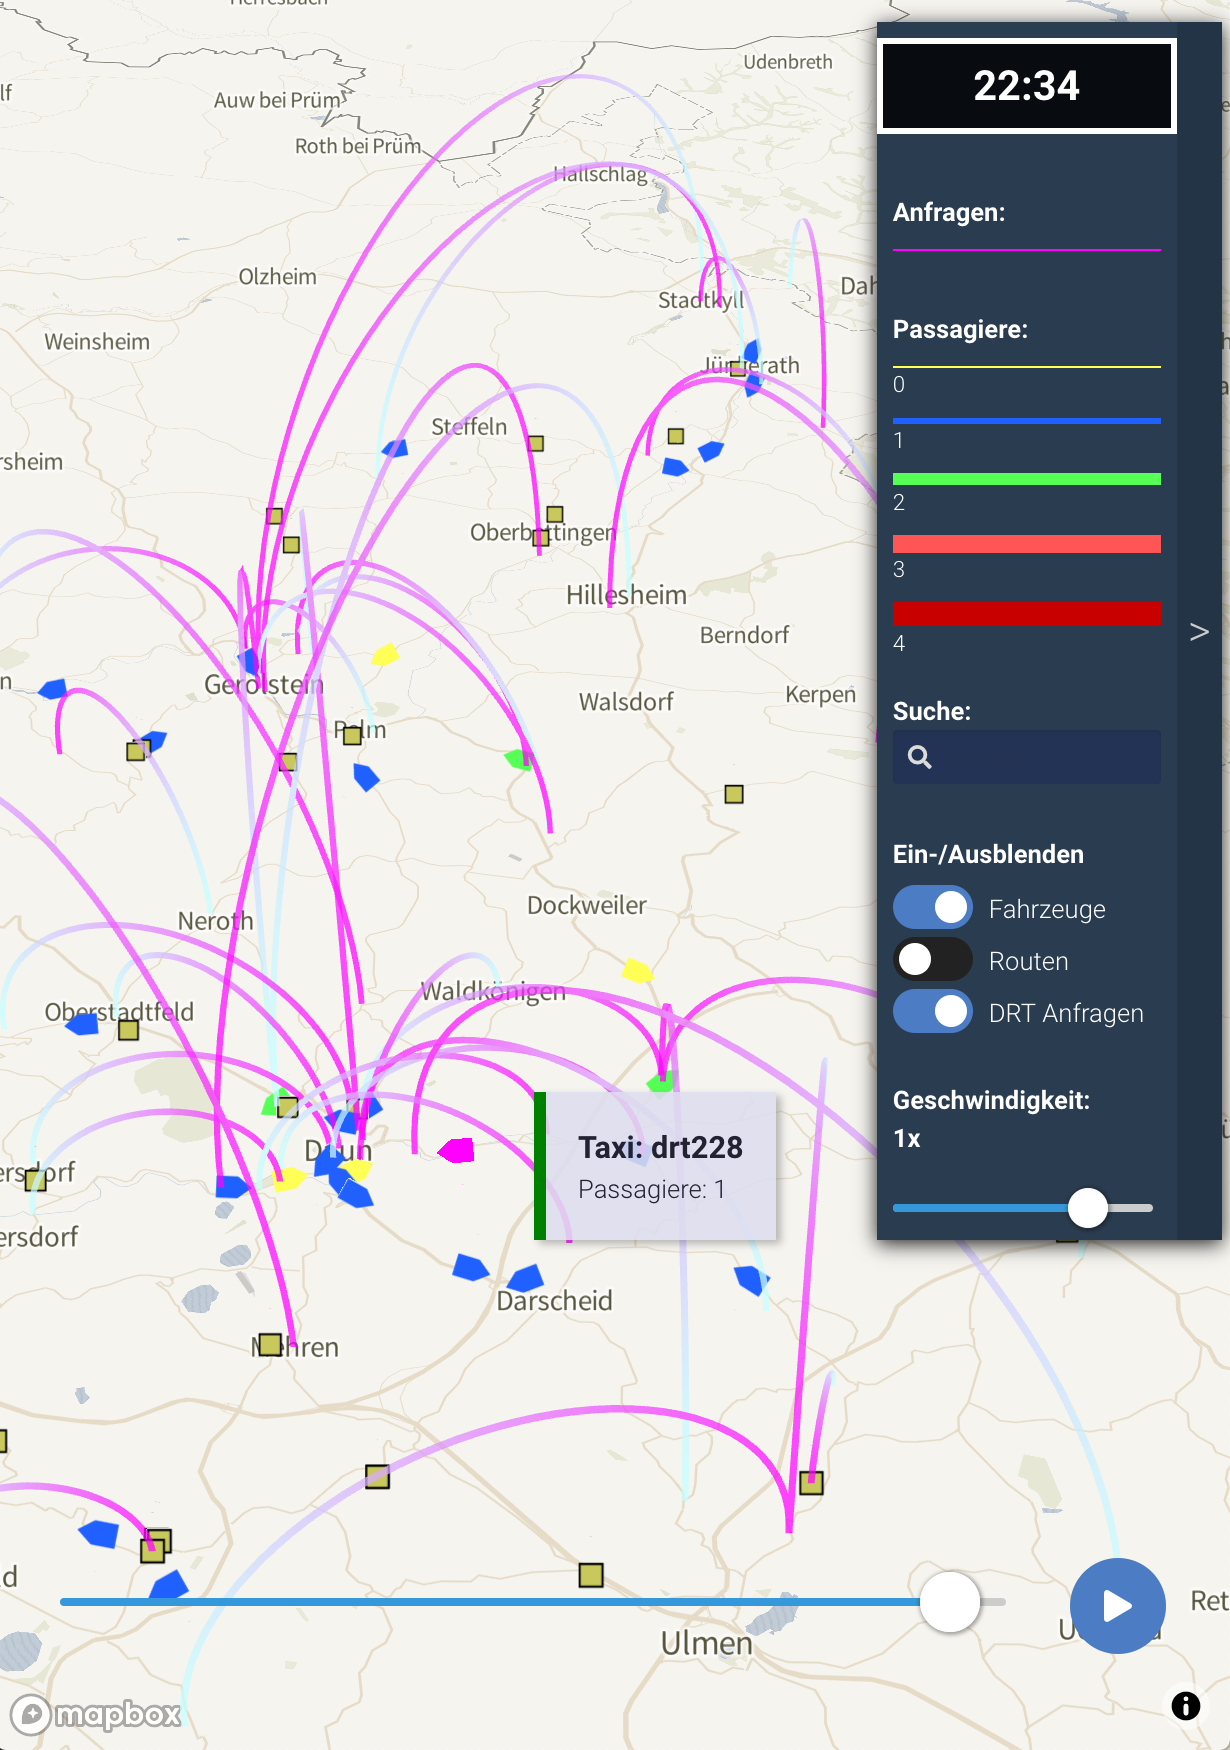
\includegraphics[width=\linewidth]{chapters/22-avov/images/fig-drt-flyovers.png}
   \caption{DRT passenger origins and destinations}
   \label{fig:avov-drt-od}
\end{minipage}
% \caption{Demand Responsive Transport (DRT) animation screenshots}
\end{figure}

% ---------------------------------------------------
\subsection{DRT Passenger and Vehicle volumes}
\label{avov-volumes}

Aggregate summaries of roadway volumes depict total DRT pasenger or vehicle volumes in the entire simulation, or for specific times of day. The user can click on a specific link to see the diurnal (time of day) distribution of trips for that link, or can modify the time window being displayed for all links from total to a specific range, such as 6 A.M. to 9 A.M. if morning commute trips are being studied.

Difference plots compare the DRT scenarios to the "base case" depicting current conditions. Figure \ref{fig:avov-vehicles-daily} shows an example vehicle volume plot, with the width of the links commensurate with volumes on each link.

\begin{figure}[ht]
  \centering
  \begin{minipage}[c]{0.45\textwidth}
     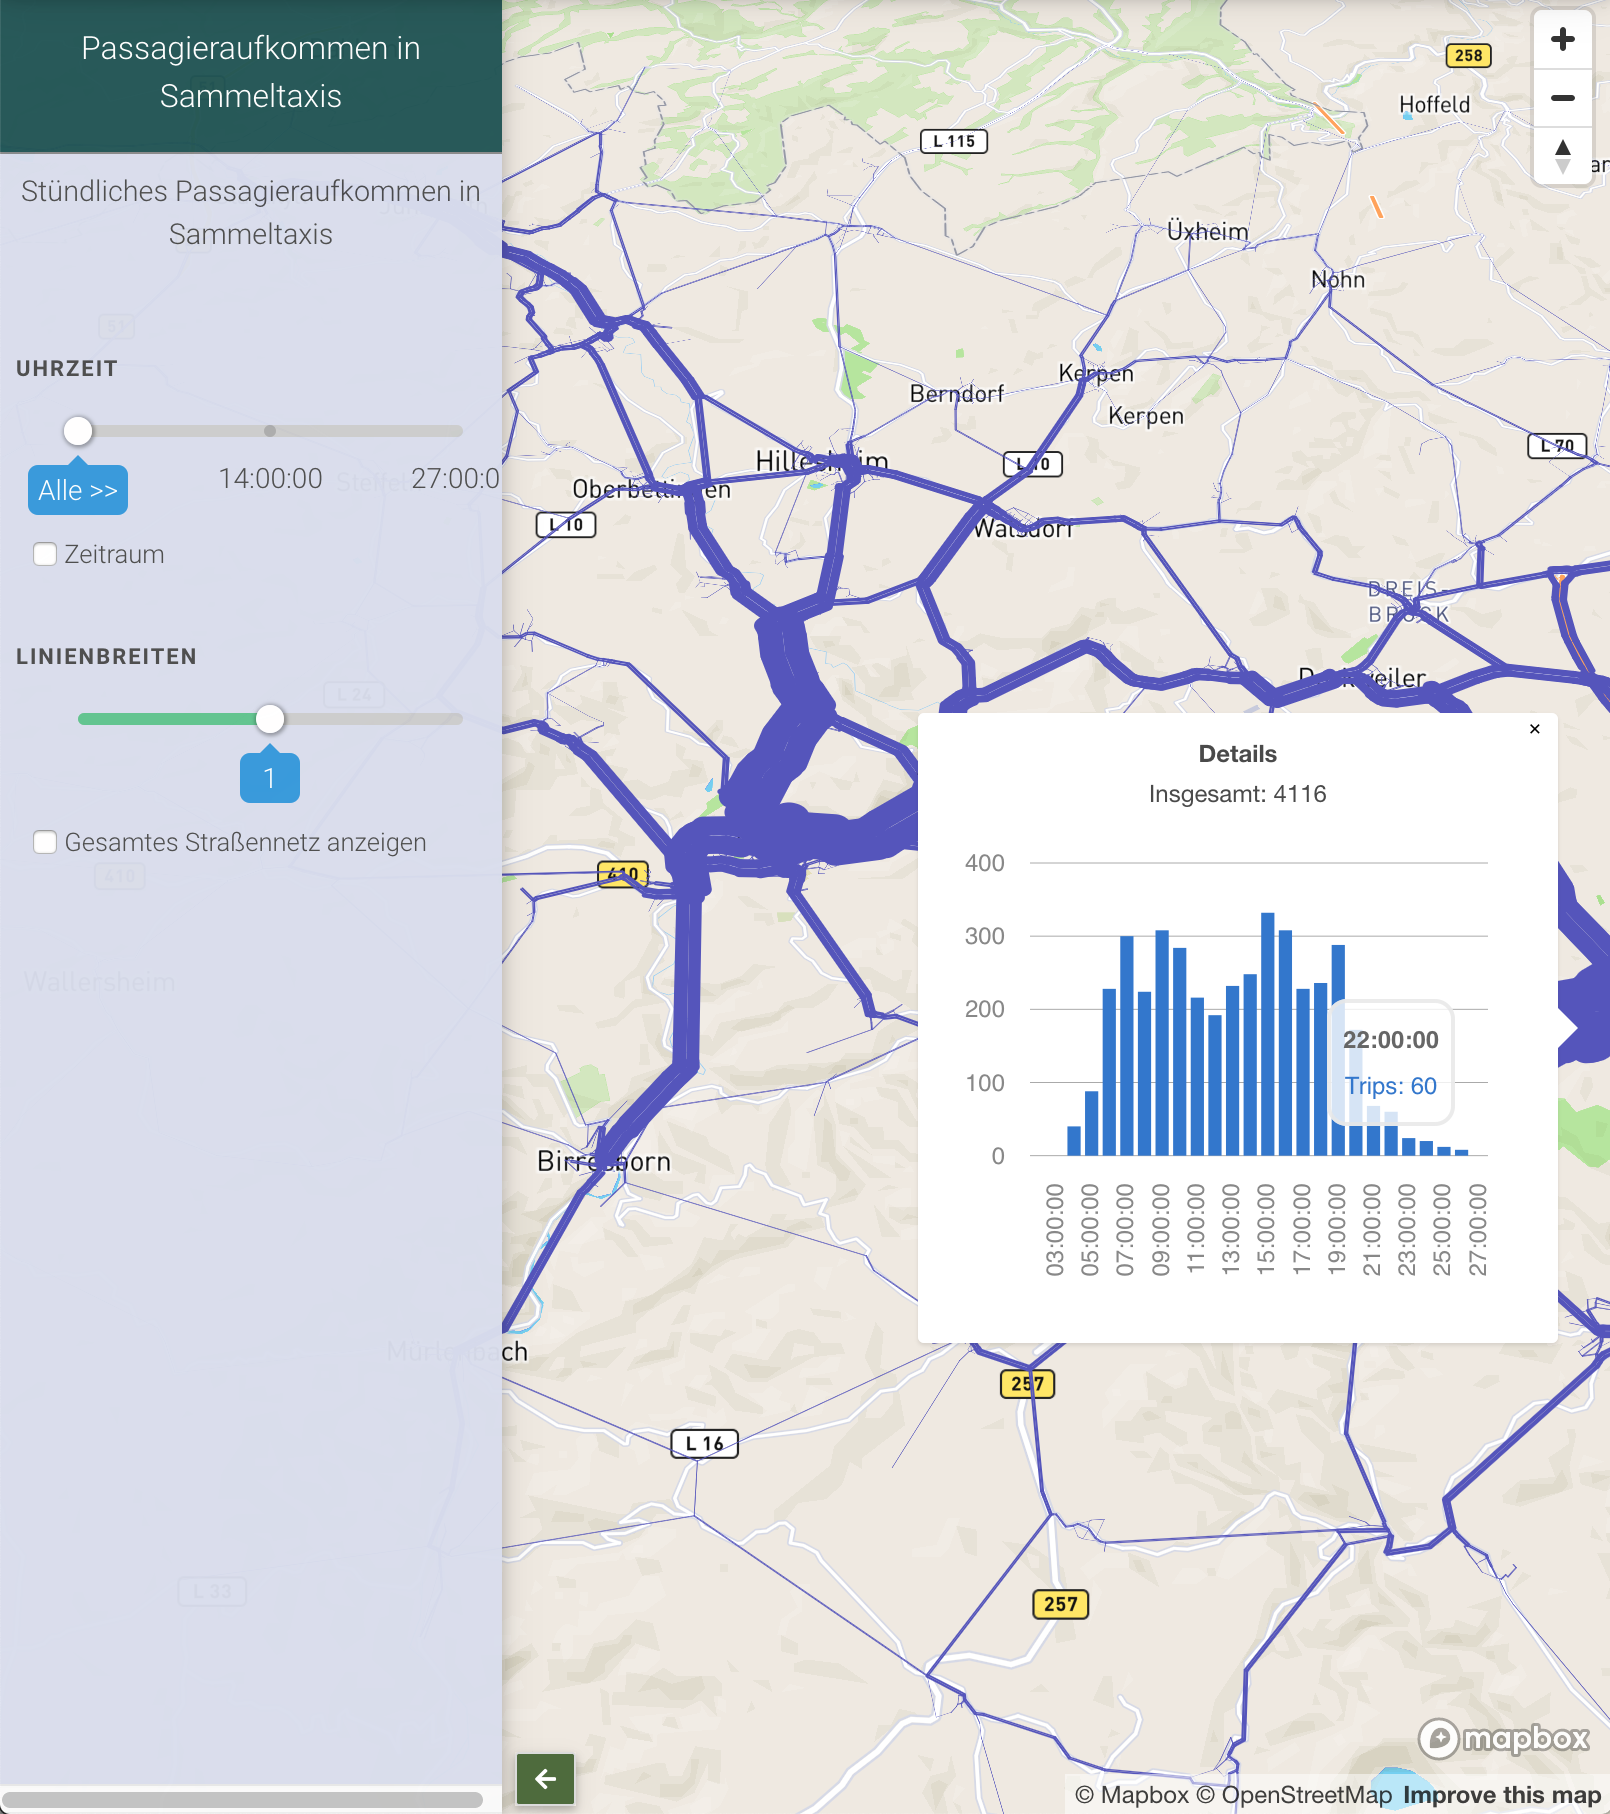
\includegraphics[width=\linewidth]{chapters/22-avov/images/fig-link-vols.png}
     \caption{DRT Vehicle volumes, daily aggregation }
     \label{fig:avov-vehicles-daily}
  \end{minipage}
  \begin{minipage}[c]{0.45\textwidth}
     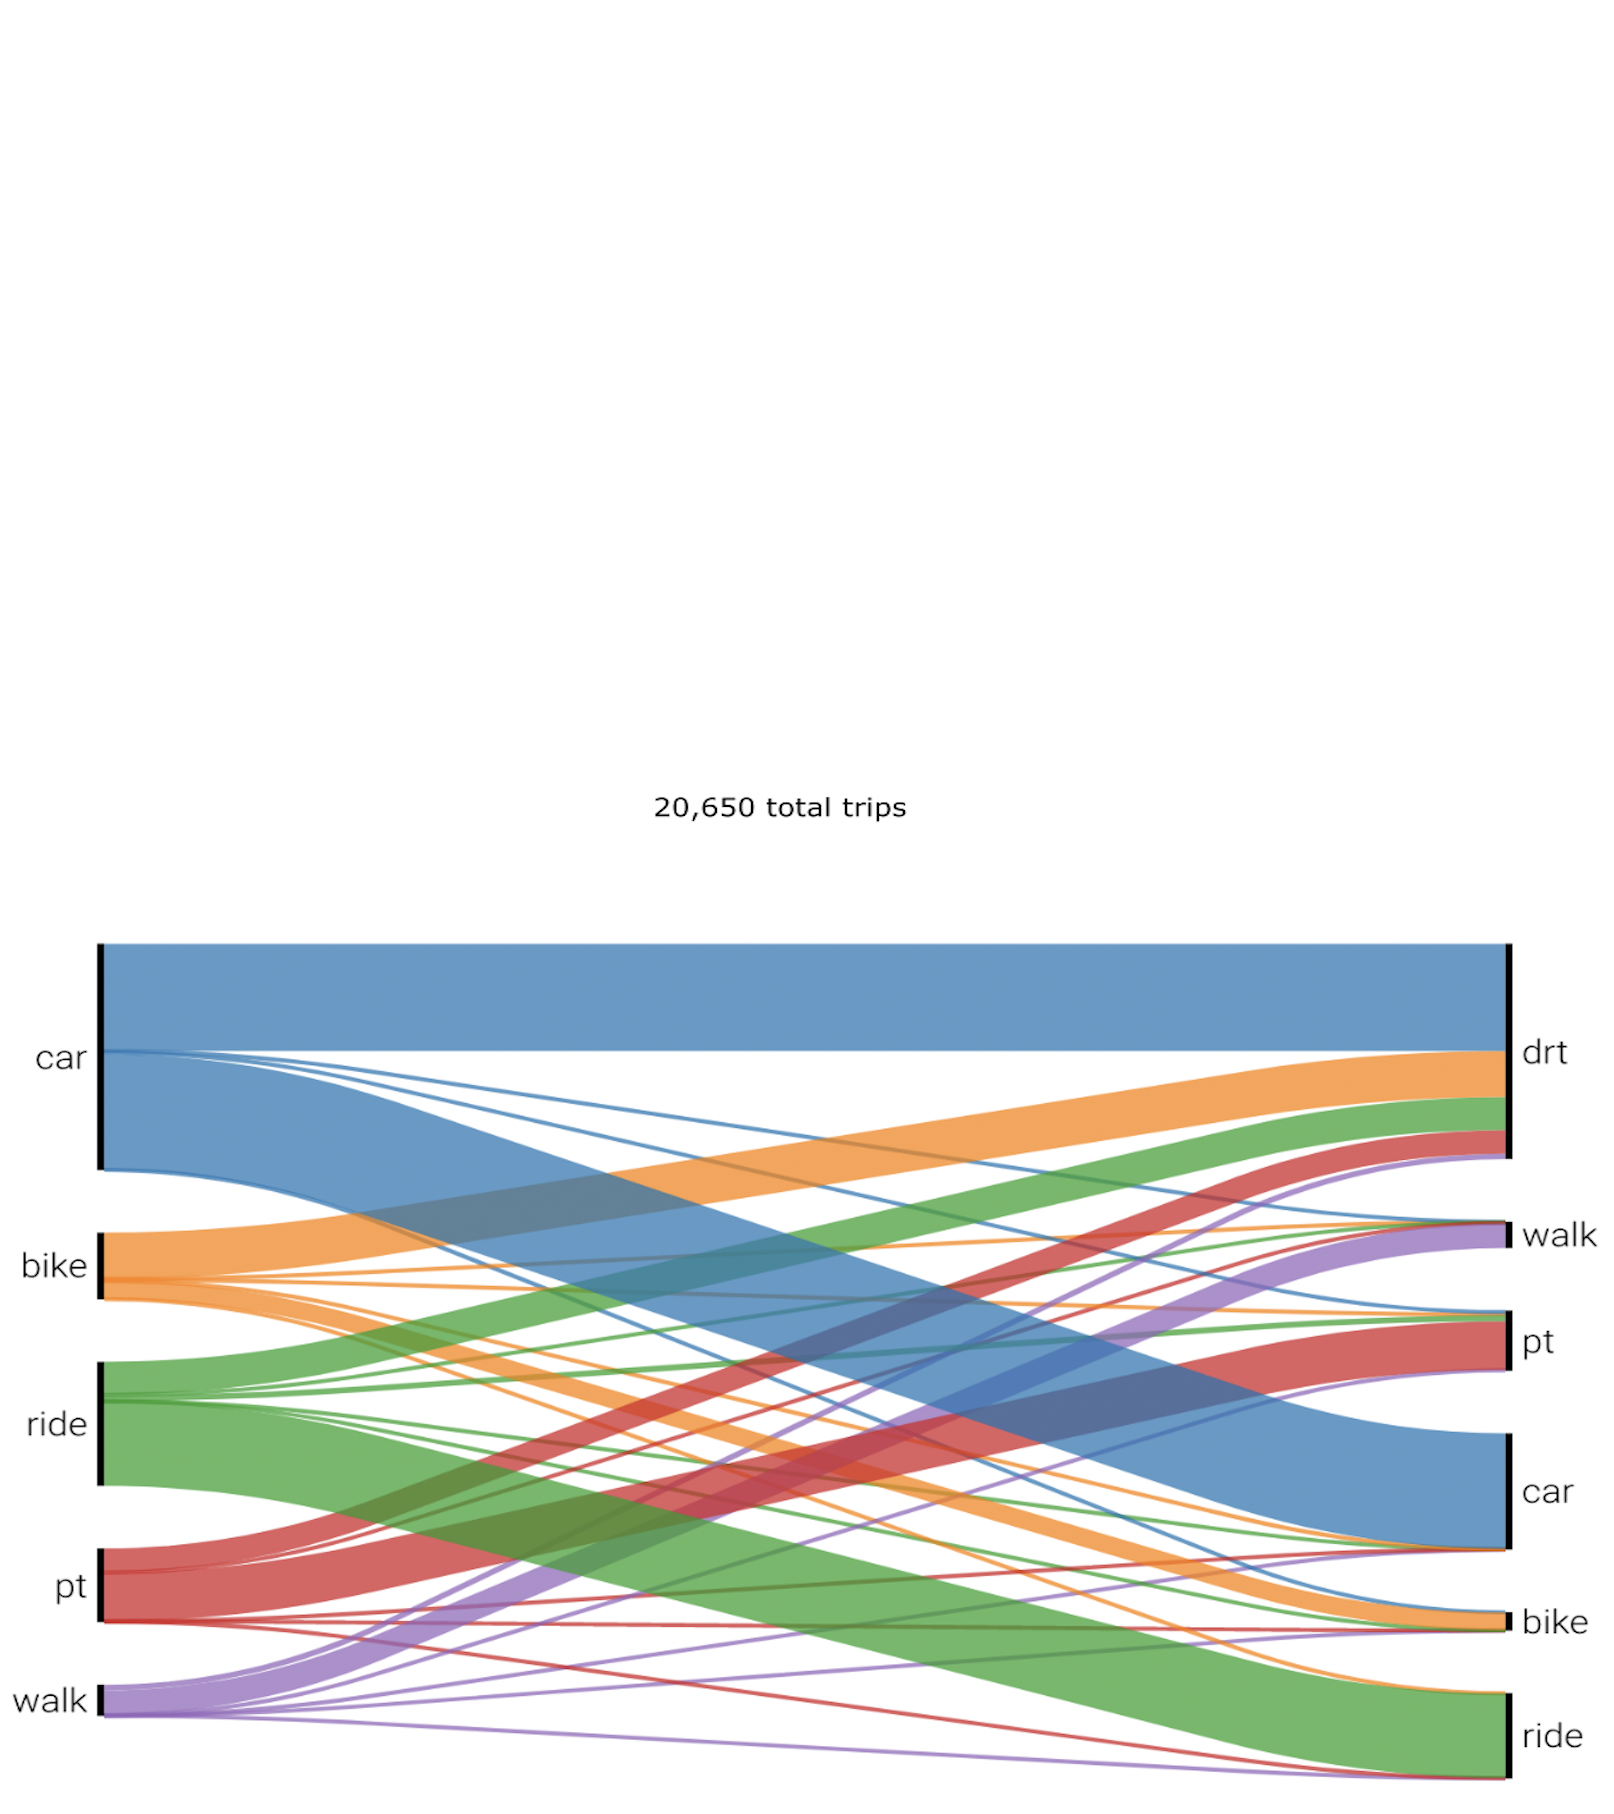
\includegraphics[width=\linewidth]{chapters/22-avov/images/fig-mode-share.png}
     \caption{Mode shift, DRT alternative vs. base case}
     \label{fig:avov-modeshift}
  \end{minipage}
  % \caption{Dynamic Response Transit (DRT) further visualization examples}
\end{figure}

% ---------------------------------------------------
\subsection{Cross-Scenario Modal Shifts}
\label{avov-mode-shifts}

Users can also \emph{compare} the aggregate total mode shift from one scenario to another; in this study comparing DRT scenarios to the base case. These visualizations highlight the degree to which the new DRT mode is "stealing" trips from existing transit and bicycle modes versus from private vehicles. Figure \ref{fig:avov-modeshift} shows an example mode shift diagram.

%% ----- RESULTS -----
\section{Results}
\label{avov-results}

Throughout summer 2020, the team iterated on dozens of DRT scenarios: varying pricing structures, presence of drivers vs. fully automated service, service coverage areas, maximum wait time goals, and so on. In August 2020 began the first public meetings with transit agency staff, with the fully operational website at \href{https://vsp.berlin/avoev}{vsp.berlin/avoev/} (available in German only).

The final site displays a front page listing the results for 6-8 scenarios in each region, covering a wide spectrum of DRT scenarios. Then for each scenario, visualizations include the individual agent animations (see above) with occupancy, origin/destination, and routing details; mode shift summaries vs. base case; vehicle volume, passenger volume, and volume differences on roadway links compared to base case; aggregate levels of tripmaking for trips originating or destined to geographical areas ("hexagon plots"); as well as detailed model output summary graphs depicting general taxi occupancy levels by time of day and more.

Each outreach meeting started with technical staff describing the study, the agent-based model, and the results for each alternative in overview; followed by small break-out groups online, in which people could explore the scenarios and discuss the findings amongs themselves; and finally a return en banc for group discussion. No problems with bugs or site performance were reported.

Some direct feedback from analysts included:

\small{

\begin{displayquote}\emph{
  The DRT viz helped us understand better how the drt code works and find some issues, e.g. when the system is congested weird things can happen and a large group of vehicles with one passenger per vehicle only moves from the same start to the same destination at the same time (in an attempt to save each passenger a few seconds it serves them separately and wastes vehicles which then are missing for the next requests). It is really nice to have requests and vehicle occupancy shown, Via did only the latter after some pre-processing.
}\end{displayquote}

\begin{displayquote}\emph{
  The website obviously made the AVÖV workshops easier. Instead of only sharing our screen we could hand out a website where people could click themselves. Unfortunately it seemed that those listeners did not use the website a lot and rather kept listening to us. Some hypotheses: Maybe because sometimes a group of people shared one computer and their internet connection was bad, maybe because they are not used to that kind of interaction...
}\end{displayquote}

\begin{displayquote}\emph{
  The other plots like passengers/link or vehicles/link are not entirely new; some used QGis to produce those. However, the website forced us to actually produce all those plots systematically instead of 'we could do that plot, but maybe it's not necessary, let's look into something else or raw data only to avoid the hassle of setting up QGis...'
}\end{displayquote}

}

The feedback that some of these visualizations are not entirely "new" is expected: tools such as QGis and Via provide some very nice visualization capabilities already. They are not online tools, however, and are not accessible to non-technical staff such as at a public outreach meeting.

Given this feedback, the initial roll-out of the visualization platform seems to have had a positive impact, and the team expects to continue developing it for further analysis of dynamic-response transit systems.

%% ----- CONCLUSIONS -----
\section{Summary}
\label{avov-summary}

Several years of trial and error led us to this specific combination of technologies and techniques. The research team is deeply indebted to the developers of so many components and libraries on which this is based, all of which are freely available online and without which this work would have been entirely impossible. The final product is more than parts merely cobbled together: a usable, useful tool for decision-making now exists, and the DRT-specific extensions serve as a template for further work.

Paraphrasing Dennis Ritchie's early description of the UNIX system in \citet{Ritchie1978unix}, ``Success lies not so much in new inventions but rather in the full exploitation of a carefully selected set of fertile ideas, and especially in showing that they can be keys to the implementation of a small yet powerful system.''

The successful experience using the platform in a public outreach setting confirms the team's expectation that advanced agent-based simulations can be part of a decision framework and public policy discussions -- ultimately leading to better-informed decisionmaking.

Further enhancements to the underlying platform and to the DRT visualization capabilities are ongoing; the plugin architecture enables other JavaScript developers to write plugins for their own agent-based models and their own use cases, if they so desire.

The website remains online at \href{https://vsp.berlin/avoev/}{vsp.berlin/avoev/}. All code is available at \href{https://github.com/matsim-vsp/avoev}{github.com/matsim-vsp/avoev/} and is licensed under the GNU GPL Version 3 \cite{FSF2007GnuGPL}. As primary author of all of the code therein, I welcome feedback and code contributions.

\section{Acknowledgements}
This research benefited from many discussions with Professor Kai Nagel, and was funded in part by the German Federal Ministry of Transport and Digital Infrastructure (funding number 16AVF2160)
